% ============================================================================
% CAPÍTULO 4 — RESULTADOS Y DISCUSIÓN
% Reconstruido el 2026-07-28. TODAS las cifras provienen de archivos de
% resultados verificables (ninguna tipeada a mano sin fuente):
%   - resultados_experimentos\exp1_binaria.csv, exp1_por_familia.csv, exp2_multiclase.csv
%   - resultados_canonicos\corrida_canonica_resumen.csv, corrida_canonica_por_familia.csv
%   - Tesis Carlos y Romina\Pruebas.xlsx (evaluación de herramientas)
% ============================================================================

Este capítulo presenta los resultados de los tres experimentos diseñados y de la evaluación de las herramientas existentes, junto con un análisis comparativo y la discusión de sus implicaciones.

\section{Pruebas Preliminares}
\label{sec:resultados_preliminares}

\subsection{Clasificación Binaria Preliminar (Fase 1)}

La Tabla~\ref{tab:res_prelim_bin} resume el desempeño de los seis modelos sobre el conjunto reducido de 350 archivos con dos características (entropía de Shannon y tamaño).

\begin{table}[ht]
\centering
\caption{Resultados preliminares de clasificación binaria (350 archivos, 2 features, partición fija)}
\label{tab:res_prelim_bin}
\begin{tabular}{|l|c|c|c|c|c|}
\hline
\textbf{Modelo} & \textbf{Exactitud (\%)} & \textbf{Precisión 0} & \textbf{Recall 0} & \textbf{Precisión 1} & \textbf{Recall 1} \\ \hline
SVM & 66,67 & 0,00 & 0,00 & 0,67 & 1,00 \\ \hline
Regresión Logística & 66,67 & 0,00 & 0,00 & 0,67 & 1,00 \\ \hline
MLP & 94,29 & 0,93 & 0,89 & 0,95 & 0,96 \\ \hline
KNN & 97,14 & 0,96 & 0,95 & 0,98 & 0,98 \\ \hline
Árbol de Decisión & 100,00 & 1,00 & 1,00 & 1,00 & 1,00 \\ \hline
Gradient Boosting & 100,00 & 1,00 & 1,00 & 1,00 & 1,00 \\ \hline
\end{tabular}
\end{table}

Los modelos lineales mostraron sesgo hacia la clase mayoritaria, mientras que los basados en árboles alcanzaron clasificación perfecta sobre la partición de prueba. Dado que esta fase no empleó validación cruzada y usó solo 350 archivos, los valores del 100\% deben interpretarse como indicio de viabilidad con posible sobreajuste, no como rendimiento esperable; la estimación rigurosa corresponde al Experimento~1 (Sección~\ref{sec:exp1}).

\subsection{Clasificación Multiclase Preliminar (Fase 2)}

Sobre el conjunto ampliado de 1.600 archivos y las seis métricas estadísticas, la exactitud multiclase resultó marginalmente superior al azar (3,2\% para 31 clases equiprobables). La Tabla~\ref{tab:res_prelim_multi} muestra la exactitud promedio utilizando métricas individuales.

\begin{table}[ht]
\centering
\caption{Exactitud promedio en clasificación multiclase preliminar con métricas individuales (31 clases)}
\label{tab:res_prelim_multi}
\begin{tabular}{|l|c|}
\hline
\textbf{Modelo} & \textbf{Exactitud promedio (\%)} \\
\hline
MLP & 7,7 \\
SVM & 7,6 \\
Regresión Logística & 7,1 \\
KNN & 5,9 \\
Random Forest & 5,4 \\
Árbol de Decisión & 5,3 \\
\hline
\end{tabular}
\end{table}

Las combinaciones de pares de métricas elevaron la exactitud hasta un 13,4\% (Random Forest, Chi-Cuadrado + correlación serial), y la aplicación de transformaciones polinomiales alcanzó un máximo de 20,5\% (MLP, Shannon-100B + correlación serial): valores muy por debajo de cualquier utilidad práctica. Este resultado motivó la formulación del Experimento~2 como validación formal del hallazgo negativo.

\section{Experimento 1: Detección Binaria de Archivos Cifrados}
\label{sec:exp1}

La Tabla~\ref{tab:exp1} presenta los resultados de detección binaria (cifrado vs.\ seguro) sobre los 1.600 archivos con las seis métricas estadísticas. Las columnas de mínimo y máximo corresponden a la variación de exactitud entre familias.

\begin{table}[ht]
\centering
\caption{Resultados de detección binaria (cifrado vs.\ seguro)}
\label{tab:exp1}
\begin{tabular}{|l|c|c|c|}
\hline
\textbf{Modelo} & \textbf{Exactitud media (\%)} & \textbf{Mínima (\%)} & \textbf{Máxima (\%)} \\ \hline
Random Forest & 88,6 & 69,3 & 97,3 \\ \hline
Gradient Boosting & 87,7 & 69,3 & 95,3 \\ \hline
Árbol de Decisión & 87,4 & 68,0 & 94,7 \\ \hline
KNN & 81,0 & 74,7 & 90,0 \\ \hline
SVM Lineal & 74,4 & 66,7 & 88,0 \\ \hline
Regresión Logística & 73,8 & 66,7 & 80,0 \\ \hline
\end{tabular}
\end{table}

Random Forest obtuvo la mejor exactitud media (88,6\%), seguido por Gradient Boosting (87,7\%). Los modelos lineales mostraron rendimiento inferior, consistente con la naturaleza no lineal de las fronteras de decisión en el espacio de métricas estadísticas.

El análisis por familia (Apéndice) revela una variación considerable: con Random Forest, la detección oscila entre el 69,3\% (RANSOMEXX) y el 97,3\% (WANNACRY). Esta variación indica que algunas familias producen archivos cifrados con propiedades estadísticas menos separables de los archivos legítimos, por ejemplo por cifrado parcial o por preservación de estructura del archivo original.

La exactitud del 88,6\% con 6 features es coherente con la literatura: Davies et al.~\cite{paper_4_comparison_of_entropy} reportaron precisiones superiores utilizando datasets más grandes y combinaciones optimizadas de métricas de entropía.

\section{Experimento 2: Clasificación Multiclase de Familias por Archivos}
\label{sec:exp2}

La Tabla~\ref{tab:exp2} presenta los resultados de clasificación multiclase (31 clases) utilizando las mismas métricas estadísticas.

\begin{table}[ht]
\centering
\caption{Resultados de clasificación multiclase por archivos (31 clases)}
\label{tab:exp2}
\begin{tabular}{|l|c|c|}
\hline
\textbf{Modelo} & \textbf{Exactitud media (\%)} & \textbf{Desvío (\%)} \\ \hline
Gradient Boosting & 9,9 & 0,5 \\ \hline
Random Forest & 9,8 & 0,9 \\ \hline
Árbol de Decisión & 9,4 & 0,6 \\ \hline
SVM Lineal & 8,7 & 0,7 \\ \hline
KNN & 7,9 & 1,2 \\ \hline
\end{tabular}
\end{table}

El mejor modelo (Gradient Boosting) alcanzó solo un 9,9\% de exactitud, apenas tres veces el azar teórico para 31 clases equiprobables (3,2\%).

La interpretación inmediata de este resultado es que los archivos cifrados por distintas familias son estadísticamente indistinguibles, lo cual es coherente con la convergencia esperada de los algoritmos criptográficos modernos: AES-256, RSA y ChaCha20 producen salidas que satisfacen las mismas propiedades de aleatoriedad, de modo que todas las familias generan entropías de Shannon próximas a 8,0 bits/byte (Figura~\ref{fig:entropia_familia}), valores de $\chi^2$ que no rechazan la uniformidad y correlaciones seriales cercanas a cero.

\begin{figure}[ht]
\centering
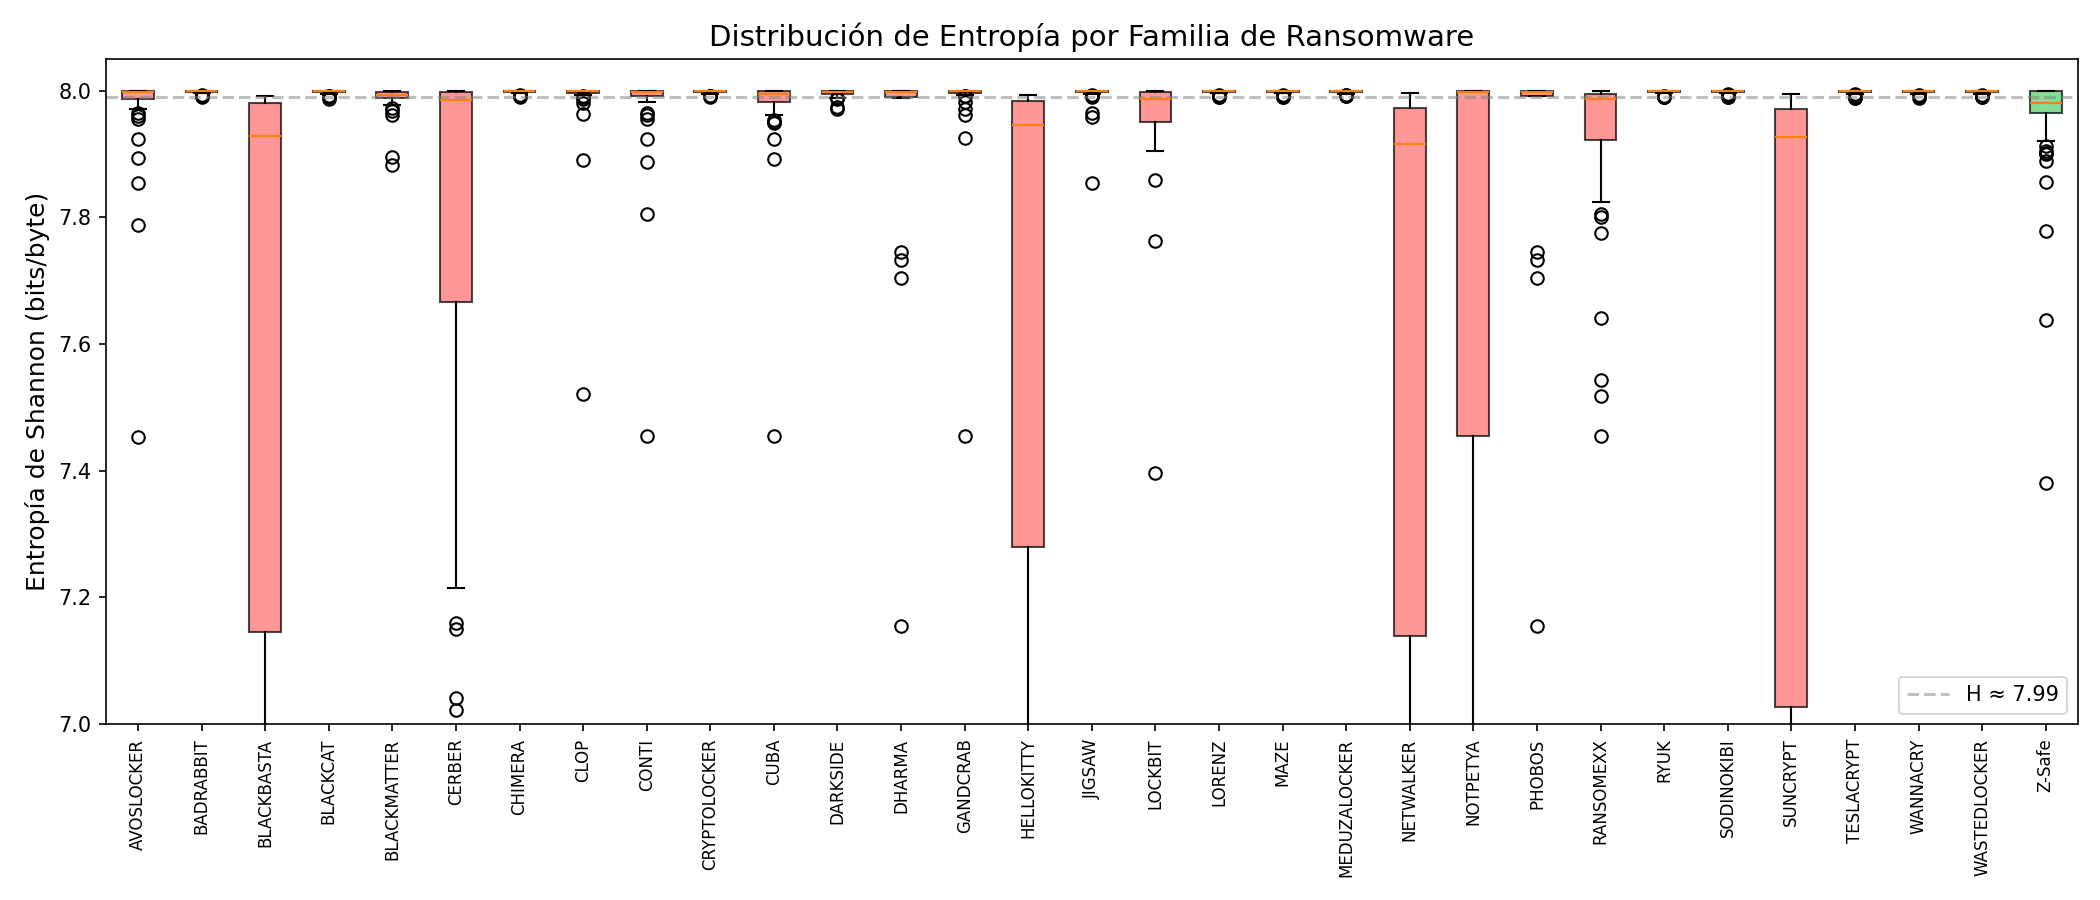
\includegraphics[width=0.95\textwidth]{images/fig_entropia_por_familia.png}
\caption{Distribución de la entropía de Shannon de los archivos cifrados por familia. La convergencia de todas las familias hacia valores próximos a 8,0 bits/byte muestra que la aleatoriedad global no discrimina.}
\label{fig:entropia_familia}
\end{figure}

Sin embargo, esta conclusión resultó ser demasiado amplia. El experimento anterior emplea únicamente dos características (entropía global y tamaño) sobre 1.600 archivos, y cabe la objeción legítima de que el resultado negativo se deba a la pobreza del espacio de representación y no a una propiedad de los datos. La Sección~\ref{subsec:exp2_ampliacion} pone a prueba esa objeción, y la respuesta obliga a reformular el hallazgo.

\subsection{Ampliación del espacio de características}
\label{subsec:exp2_ampliacion}

Para descartar que la baja exactitud fuera un artefacto de un espacio de representación insuficiente, se repitió el experimento sobre el conjunto completo de NapierOne-\textit{small}~\cite{paper_7_napierone} ---29.029 archivos, 1.001 por cada una de las 29 familias disponibles--- ampliando de 2 a \textbf{275 características} por archivo. Además de las métricas estadísticas globales ya descritas, se incorporaron: entropía calculada por regiones (cabecera, cola y bloques intermedios), desvío estándar de la entropía entre bloques, diferencia de entropía entre cabecera y cola, longitud de la racha más larga de bytes repetidos, proporción de bytes nulos y de caracteres imprimibles, número de bytes distintos, y la distribución completa de frecuencia de los 256 valores de byte posibles.

Se evaluaron cinco subconjuntos de características con tres algoritmos, mediante validación cruzada estratificada de 5 particiones. Se empleó \texttt{HistGradientBoostingClassifier} en lugar del \textit{Gradient Boosting} clásico porque, con 29 clases, este último requiere entrenar $n_{\text{clases}} \times n_{\text{estimadores}} = 2.900$ árboles por ajuste, lo que resulta computacionalmente inviable sobre 29.000 muestras; la implementación basada en histogramas es el equivalente recomendado para conjuntos con más de 10.000 muestras~\cite{sklearn}. Los resultados se presentan en la Tabla~\ref{tab:exp2_ampliado}.

\begin{table}[ht]
\centering
\caption{Exactitud multiclase (29 familias) según el subconjunto de características. Validación cruzada de 5 particiones sobre 29.029 archivos. Azar $= 0{,}034$.}
\label{tab:exp2_ampliado}
\begin{tabular}{|l|c|c|c|}
\hline
\textbf{Subconjunto de características} & \textbf{Random Forest} & \textbf{KNN-5} & \textbf{HistGB} \\
\hline
Entropía global + tamaño (2) & 0,166 & 0,126 & 0,163 \\
Estadísticas globales (9) & 0,391 & 0,300 & 0,399 \\
Frecuencia de bytes (256) & 0,184 & 0,082 & 0,199 \\
Todas las características (275) & 0,542 & 0,143 & 0,592 \\
\textbf{Estadísticas + derivadas (19)} & \textbf{0,603} & 0,299 & 0,598 \\
\hline
\end{tabular}
\end{table}

El resultado es inequívoco: con un espacio de representación adecuado la exactitud pasa de 0,166 a \textbf{0,603}, casi dieciocho veces el azar. La afirmación de que las propiedades estadísticas no permiten distinguir familias, tal como se formuló a partir del experimento inicial, es incorrecta.

Conviene precisar que estos valores se obtuvieron con la configuración por defecto de cada algoritmo, sin búsqueda de hiperparámetros. La optimización se reservó para las dos configuraciones que resultaron determinantes ---el clasificador sobre bytes (Sección~\ref{sec:exp2c}) y el clasificador de notas (Sección~\ref{subsec:exp3_hiperparametros})--- por dos motivos: el propósito de este experimento es delimitar el alcance del resultado negativo inicial, para lo cual basta demostrar que la exactitud crece sustancialmente al ampliar la representación; y el valor aquí obtenido queda superado por el del Experimento 2c sobre el mismo conjunto de datos, de modo que una optimización adicional no alteraría las conclusiones. Se señala como limitación explícita del alcance de este experimento.

Dos observaciones secundarias merecen registrarse. En primer lugar, las 275 características (0,592) rinden ligeramente \textit{peor} que 19 seleccionadas por criterio experto (0,603): las 256 frecuencias de byte introducen ruido sin aportar señal, un caso claro de maldición de la dimensionalidad. En segundo lugar, la selección automática por prueba F de ANOVA no mejora ese resultado (0,363 con 10 características, 0,387 con 50), lo que confirma que el aporte proviene de la interacción entre características y no de unas pocas individualmente dominantes.

\subsection{Dónde reside la información discriminante}
\label{subsec:exp2_donde}

El análisis de importancia de características del Random Forest~\cite{breiman2001} explica el resultado anterior y constituye, a juicio de este trabajo, el hallazgo conceptual más relevante del frente de archivos cifrados. La Tabla~\ref{tab:exp2_importancias} presenta las diez características más informativas.

\begin{table}[ht]
\centering
\caption{Características más discriminativas según la importancia de Gini del Random Forest}
\label{tab:exp2_importancias}
\begin{tabular}{|c|l|c|l|}
\hline
\textbf{\#} & \textbf{Característica} & \textbf{Importancia} & \textbf{Qué mide} \\
\hline
1 & \texttt{longest\_run} & 0,0715 & Racha más larga de bytes repetidos \\
2 & \texttt{entropy\_diff\_hf} & 0,0412 & Diferencia de entropía cabecera--cola \\
3 & \texttt{entropy\_footer} & 0,0402 & Entropía de la cola del archivo \\
4 & \texttt{entropy\_header} & 0,0314 & Entropía de la cabecera \\
5 & \texttt{chi\_square} & 0,0148 & Estadístico $\chi^2$ global \\
6 & \texttt{zero\_ratio} & 0,0111 & Proporción de bytes nulos \\
7 & \texttt{byte\_freq\_000} & 0,0108 & Frecuencia del byte \texttt{0x00} \\
8 & \texttt{file\_size} & 0,0095 & Tamaño del archivo \\
9 & \texttt{block\_entropy\_std} & 0,0081 & Variación de entropía entre bloques \\
10 & \texttt{byte\_freq\_max} & 0,0074 & Frecuencia del byte más común \\
\hline
\end{tabular}
\end{table}

Ninguna de las características dominantes mide la calidad criptográfica del cifrado. Todas miden, de una u otra forma, \textbf{la presencia de datos no aleatorios dentro de un archivo por lo demás aleatorio}: rachas de bytes repetidos, asimetría de entropía entre el comienzo y el final, exceso de bytes nulos, variación de entropía entre bloques. Son indicadores indirectos de que la familia ha añadido una cabecera, una cola o un bloque de relleno al contenido cifrado.

Esto reformula el resultado del Experimento 2 en los siguientes términos, que son los que este trabajo sostiene:

\begin{quote}
La información que permite distinguir familias de ransomware a partir de sus archivos cifrados no reside en las propiedades criptográficas del contenido ---que son, en efecto, indistinguibles--- sino en la \textbf{estructura} del archivo: en los artefactos no aleatorios que cada familia añade deliberadamente. Medida globalmente, la aleatoriedad no discrimina (0,166); medida por regiones y rachas, alcanza 0,603.
\end{quote}

Esta lectura es además coherente con la capacidad de ID Ransomware de identificar el 66,67\% de las familias a partir de archivos cifrados (Sección~\ref{sec:res_herramientas}): la herramienta no emplea estadística sino firmas de bytes en posiciones conocidas. Las dos secciones siguientes ponen a prueba esta hipótesis de forma directa, primero localizando explícitamente esas firmas (Experimento 2b) y luego aprendiéndolas de los datos (Experimento 2c).

\section{Experimento 2b: Identificación por Artefactos Estructurales}
\label{sec:exp2b}

\subsection{Motivación y diseño}

Dos observaciones independientes motivaron este experimento. La primera surgió de la evaluación de herramientas descrita en la Sección~\ref{sec:res_herramientas}: de las veinte familias que ID Ransomware~\cite{idransomware} identifica correctamente a partir de un archivo cifrado, nueve mantienen la identificación aun cuando el archivo se renombra, lo que implica necesariamente que la evidencia utilizada está en el contenido y no en el nombre. La segunda proviene de la literatura: Davies et al.~\cite{davies2023majority} incorporan una prueba de \textit{magic number} a su sistema de detección por votación mayoritaria, alcanzando 0,961 de exactitud en la tarea binaria, lo que confirma que las firmas de bytes son un indicador explotable.

Ambas fuentes utilizan, sin embargo, catálogos de firmas construidos manualmente. El experimento aquí propuesto invierte el procedimiento: en lugar de partir de una lista conocida, las firmas se \textbf{descubren automáticamente a partir de los datos}. Para cada familia se calcula el prefijo y el sufijo binario común a todos sus archivos (el mayor prefijo y sufijo comunes sobre una ventana de 64 bytes) y la extensión añadida común. Una familia se considera estructuralmente identificable si posee un prefijo o sufijo común de al menos 4 bytes, o una extensión propia.

La clasificación se evalúa mediante el procedimiento \textit{leave-one-out}: para cada archivo, las marcas de todas las familias se recalculan excluyendo ese archivo, de modo que la predicción nunca se apoya en información derivada de la muestra evaluada. Se evaluaron 1.450 archivos (50 por familia).

\subsection{Marcas descubiertas}

El procedimiento identificó marcas estructurales en \textbf{25 de las 29 familias}. En quince casos se trata de firmas binarias en el contenido, varias de ellas legibles como texto: WANNACRY escribe \texttt{57 41 4E 41 43 52 59 21} al inicio de cada archivo, secuencia que corresponde a la cadena \texttt{WANACRY!}; CUBA inserta \texttt{FIDEL.CA} en los primeros veinte bytes; PHOBOS añade \texttt{LOCK96} al final. Otras familias emplean firmas extensas no textuales: CERBER, LOCKBIT, RANSOMEXX y TESLACRYPT presentan bloques constantes de 64 bytes.

Este resultado valida de forma independiente las anotaciones manuales realizadas durante la evaluación de ID Ransomware: las nueve familias cuya identificación sobrevivía al renombrado figuran entre las que el procedimiento automático detecta con firma binaria.

Cuatro familias ---BADRABBIT, JIGSAW, NOTPETYA y SUNCRYPT--- no presentan marca alguna. El caso de NOTPETYA coincide con lo documentado por Davies et al.~\cite{davies2023majority}, quienes observan que esta familia no modifica la extensión de los archivos que ataca y que, por ese motivo, evade las pruebas basadas en nombre y extensión. La convergencia entre ambos trabajos, obtenida por vías metodológicas distintas, refuerza la validez del procedimiento.

\subsection{Resultados y ablación}

Un resultado agregado del 86,2\% de exactitud podría atribuirse por completo a la extensión del archivo, que es también el mecanismo que emplean las herramientas basadas en reglas. Para separar ambas contribuciones se repitió la evaluación en tres modalidades (Tabla~\ref{tab:exp2b}).

\begin{table}[ht]
\centering
\caption{Ablación del Experimento 2b: contribución de cada tipo de marca (1.450 archivos, 29 familias, \textit{leave-one-out})}
\label{tab:exp2b}
\begin{tabular}{|l|c|c|c|}
\hline
\textbf{Modalidad} & \textbf{Cobertura} & \textbf{Exactitud global} & \textbf{Exactitud donde aplica} \\
\hline
Solo extensión del archivo & 82,8\% & 0,828 & 1,000 \\
Solo firmas binarias & 53,3\% & 0,517 & 0,970 \\
Combinado & 87,8\% & 0,862 & 0,982 \\
\hline
\end{tabular}
\end{table}

La interpretación de estas cifras exige cautela. La extensión acierta el 100\% de los casos en que está presente, pero ese valor perfecto es un indicio de artefacto y no de mérito: en NapierOne cada familia está representada por una única campaña, de modo que su extensión es constante dentro del conjunto de datos. En la práctica, familias como DHARMA emplean extensiones que incorporan un identificador de la víctima, por lo que la extensión constituye un identificador de \textit{campaña} y no de \textit{familia}. Su rendimiento no es extrapolable.

Las firmas binarias, en cambio, constituyen evidencia de contenido: son marcadores que el propio programa escribe en el archivo para reconocer posteriormente lo que ya ha cifrado, y por lo tanto resultan más estables entre campañas que la extensión. Alcanzan un 97,0\% de acierto, pero solo cubren el 53,3\% de los archivos: la regla de coincidencia exacta exige que la firma sea idéntica en \textit{todos} los archivos de la familia, y un único caso divergente la elimina. Esta limitación de cobertura es la que motiva el experimento siguiente.

\section{Experimento 2c: Aprendizaje Automático sobre la Estructura de Bytes}
\label{sec:exp2c}

\subsection{Motivación y diseño}

El Experimento 2b localizó la información discriminante pero la explotó mediante reglas de coincidencia exacta, con la consiguiente pérdida de cobertura. Este experimento sustituye la regla por un clasificador entrenado sobre los mismos datos, con tres objetivos: alcanzar cobertura total, tolerar variabilidad parcial en las marcas, y determinar si existe información aprovechable en las familias donde la regla exacta no encontró nada.

Se extraen los \textbf{512 primeros y 512 últimos bytes} de cada archivo. De forma deliberada, \textbf{no se utiliza el nombre ni la extensión}: dado que el Experimento 2b mostró que la extensión identifica la campaña, restringir la entrada al contenido permite medir qué información reside efectivamente en los bytes.

Se compararon dos representaciones, análogas a las empleadas con las notas de rescate:

\begin{itemize}
\item \textbf{Posicional}: los 1.024 bytes como valores en posiciones fijas. Captura marcas ancladas a desplazamientos determinados. Se emplean modelos basados en árboles, que particionan por valor exacto; se descartó el uso de modelos lineales sobre esta representación porque los valores de byte son categóricos y no ordinales, de modo que la relación de orden que un modelo lineal presupone carece de sentido.
\item \textbf{N-gramas de bytes}: los mismos bytes tratados como una secuencia de símbolos, con ponderación TF-IDF de n-gramas. Captura marcas en posición variable, y constituye el análogo directo de los n-gramas de caracteres empleados en el Experimento 3.
\end{itemize}

La selección de hiperparámetros se realizó mediante búsqueda aleatorizada \textbf{anidada}: la búsqueda se ejecuta dentro del subconjunto de entrenamiento de cada partición externa, de modo que la métrica reportada no está sesgada por el proceso de selección. La búsqueda empleó una submuestra estratificada de 5.800 archivos (200 por familia) y la mejor configuración se reevaluó sobre 14.500 archivos (500 por familia) con validación cruzada de 5 particiones.

\subsection{Resultados}

\begin{table}[ht]
\centering
\caption{Experimento 2c: clasificación mediante aprendizaje sobre bytes de cabecera y cola. Cobertura del 100\% en todas las configuraciones. Sin uso de nombre ni extensión.}
\label{tab:exp2c}
\begin{tabular}{|l|c|c|c|}
\hline
\textbf{Configuración} & \textbf{Archivos} & \textbf{Exactitud} & \textbf{Macro-F1} \\
\hline
Posicional + Random Forest (búsqueda) & 5.800 & 0,897 & 0,897 \\
N-gramas de bytes + Regresión Logística & 5.800 & 0,856 & 0,858 \\
N-gramas de bytes + LinearSVC & 5.800 & 0,849 & 0,846 \\
\hline
\textbf{Posicional + Random Forest (final)} & \textbf{14.500} & \textbf{0,910} & \textbf{0,908} \\
\hline
\end{tabular}
\end{table}

La mejor configuración alcanza una \textbf{exactitud de 0,910 y un macro-F1 de 0,908 sobre 29 familias, con cobertura total y utilizando exclusivamente el contenido del archivo}. Los hiperparámetros seleccionados fueron 300 árboles, profundidad máxima 20, mínimo de 2 muestras por hoja y 30\% de características por división.

Resulta significativo que la representación posicional supere a los n-gramas de bytes: las marcas se encuentran en \textbf{desplazamientos fijos} del archivo, coherente con cabeceras y colas escritas por el programa en posiciones determinísticas. Este comportamiento contrasta con el observado en las notas de rescate, donde los n-gramas de caracteres resultan la mejor representación; la diferencia refleja la naturaleza distinta de ambos artefactos, uno generado por código y el otro redactado por personas.

\subsection{Análisis por familia}

La Figura~\ref{fig:f1_bytes} presenta el F1 obtenido por cada familia, distinguiendo qué tipo de marca había detectado el Experimento 2b.

\begin{figure}[ht]
\centering
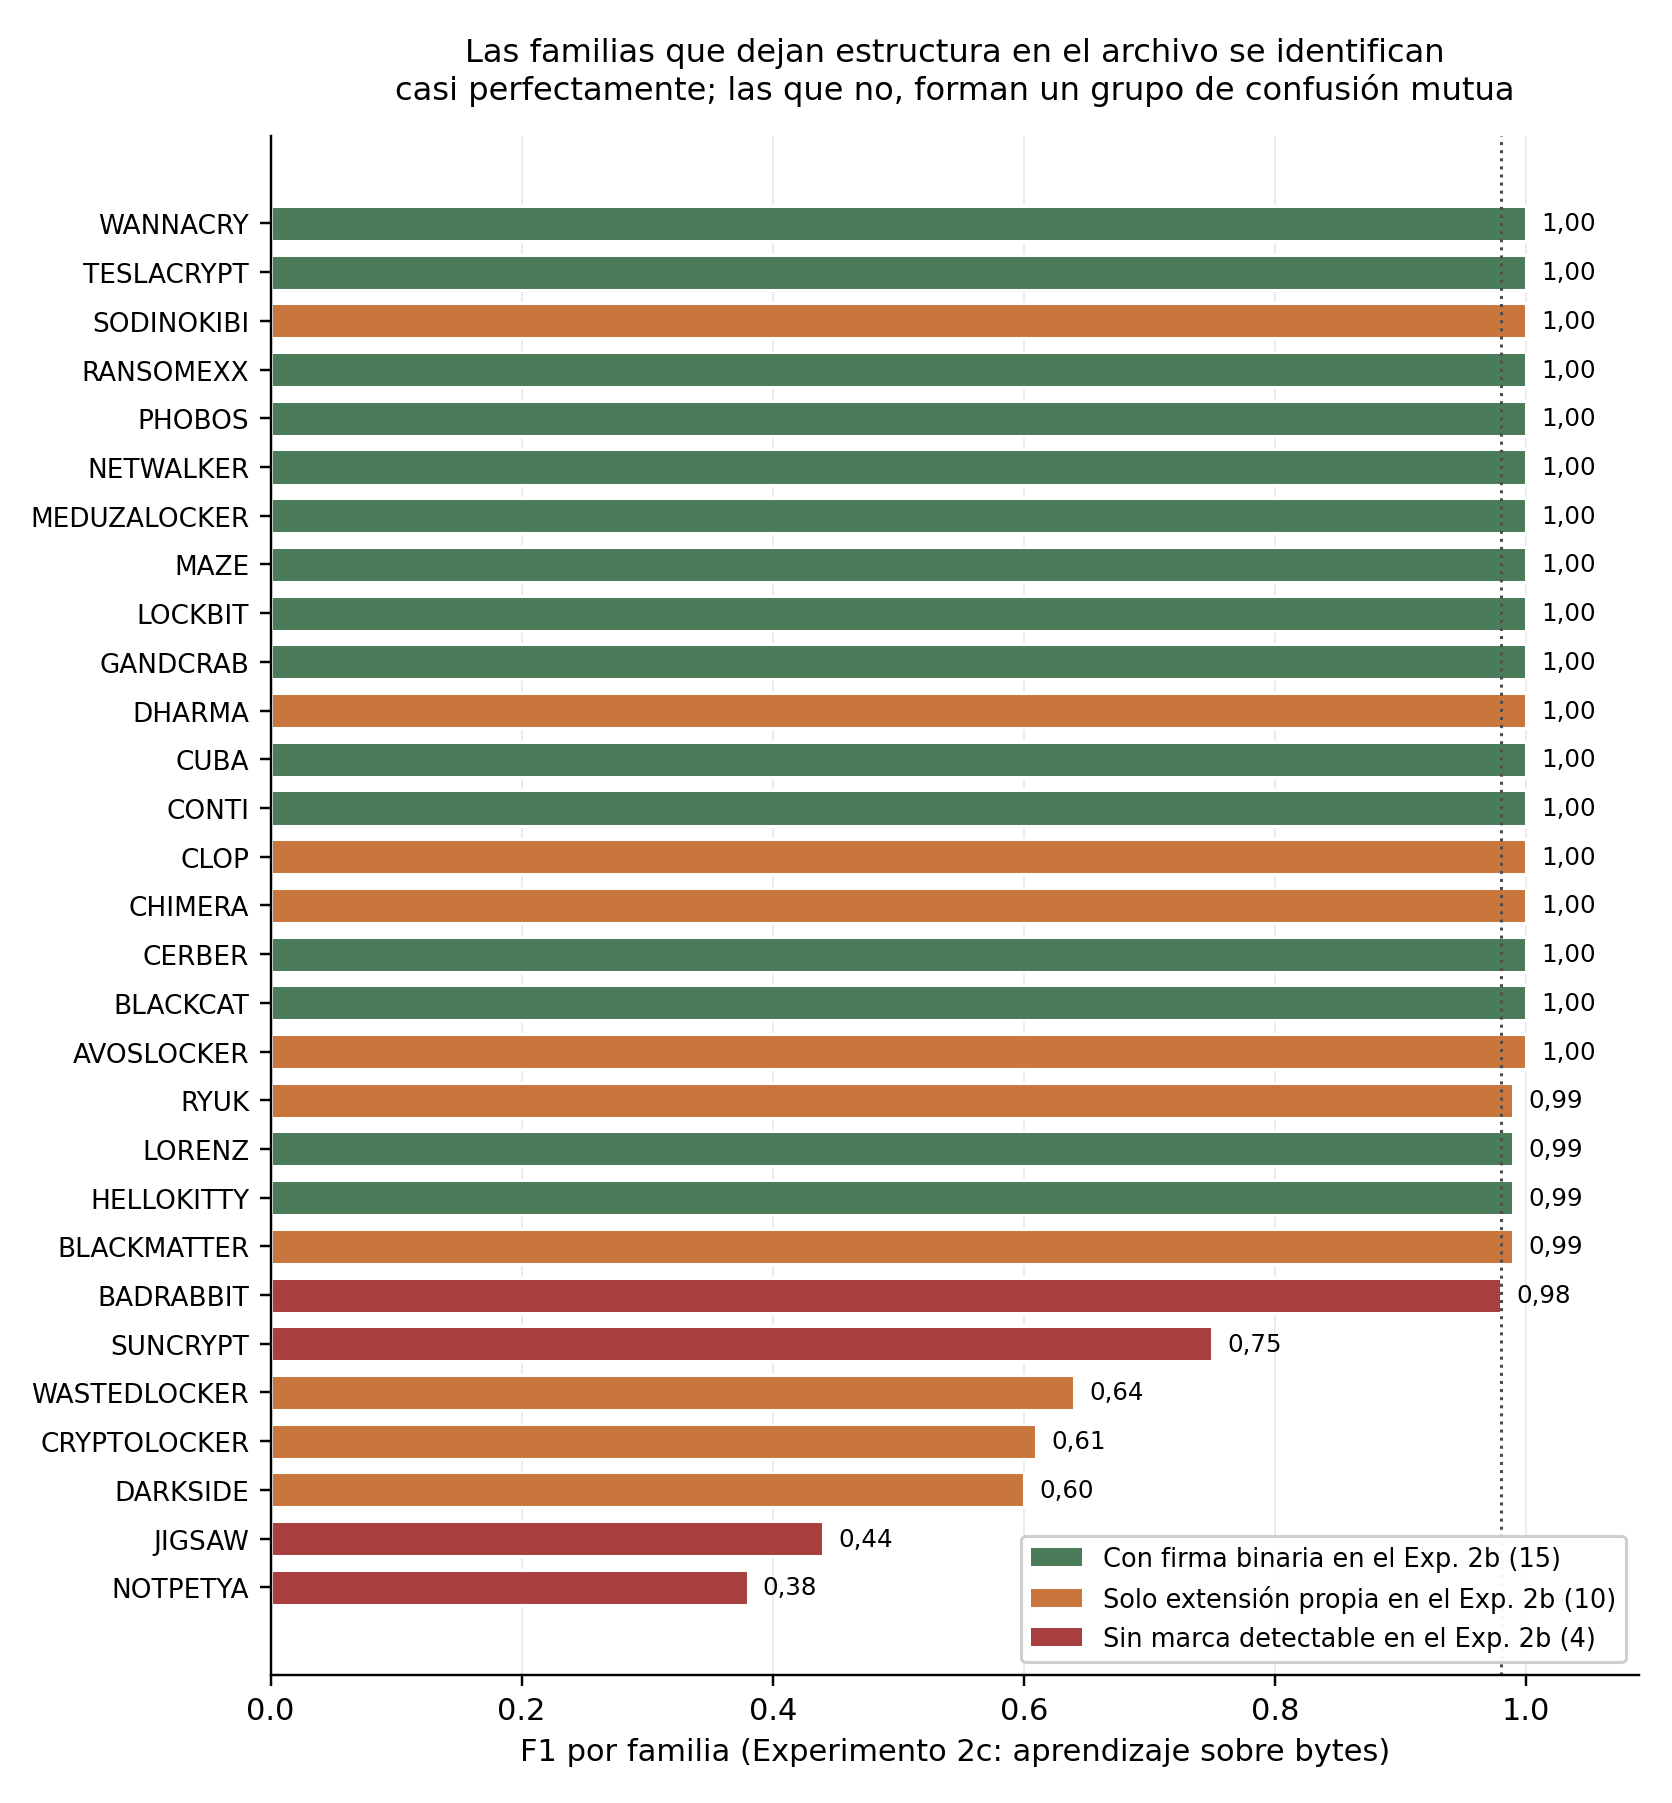
\includegraphics[width=0.86\textwidth]{images/fig_f1_por_familia_bytes.png}
\caption{F1 por familia en el Experimento 2c. El color indica el tipo de marca detectada por el Experimento 2b. Las quince familias con firma binaria se identifican sin excepción por encima de 0,99; siete de las diez que solo poseían extensión propia también, lo que indica que el clasificador halla patrones de contenido que la regla de coincidencia exacta no detecta.}
\label{fig:f1_bytes}
\end{figure}

El resultado es marcadamente bimodal: \textbf{23 de las 29 familias alcanzan un F1 igual o superior a 0,98}, mientras que seis quedan por debajo de 0,76. La correspondencia con el Experimento 2b es notable y opera como validación cruzada entre ambos:

\begin{itemize}
\item Las \textbf{quince familias con firma binaria} identificada en el Experimento 2b obtienen, sin una sola excepción, un F1 igual o superior a 0,99.
\item De las \textbf{diez familias que solo poseían extensión propia} ---es decir, sin marca detectable en el contenido mediante coincidencia exacta---, siete alcanzan igualmente valores superiores a 0,99. El clasificador extrae de los bytes información que la regla exacta no capturaba.
\item De las \textbf{cuatro familias sin marca alguna}, BADRABBIT pasa de un F1 de 0,15 en el experimento estadístico a \textbf{0,98}, quedando plenamente resuelta. SUNCRYPT (0,75), NOTPETYA (0,38) y JIGSAW (0,44) mejoran respecto de los experimentos previos pero permanecen entre las difíciles.
\end{itemize}

Las seis familias con menor rendimiento ---SUNCRYPT (0,75), WASTEDLOCKER (0,64), CRYPTOLOCKER (0,61), DARKSIDE (0,60), JIGSAW (0,44) y NOTPETYA (0,38)--- forman un grupo de confusión mutua. DARKSIDE presenta un patrón revelador: precisión de 0,45 frente a un recall de 0,90, lo que indica que actúa como clase de destino por defecto para los archivos que el modelo no logra atribuir. Estas seis familias son, presumiblemente, las que cifran sin añadir estructura al archivo, y constituyen el residuo genuino de la indistinguibilidad estadística planteada en el Experimento 2.

\subsection{Limitación}
\label{subsec:exp2c_limitacion}

El conjunto NapierOne representa cada familia mediante una única campaña, obtenida ejecutando una muestra concreta del ransomware. En consecuencia, el valor de 0,910 mide la capacidad de identificar \textit{esa campaña}, y no puede afirmarse que se extienda a campañas futuras de la misma familia, que podrían modificar sus cabeceras o colas. Esta limitación es análoga a la observada en el corpus de notas de rescate, donde la baja variabilidad de plantillas produce el mismo efecto (Sección~\ref{subsec:res_variabilidad}), y su evaluación requeriría un conjunto de datos con múltiples campañas por familia, no disponible en la actualidad.

\section{Síntesis del Frente de Archivos Cifrados}
\label{sec:sintesis_archivos}

La Figura~\ref{fig:progresion} resume la progresión de los cuatro enfoques evaluados sobre el mismo conjunto de archivos cifrados.

\begin{figure}[ht]
\centering
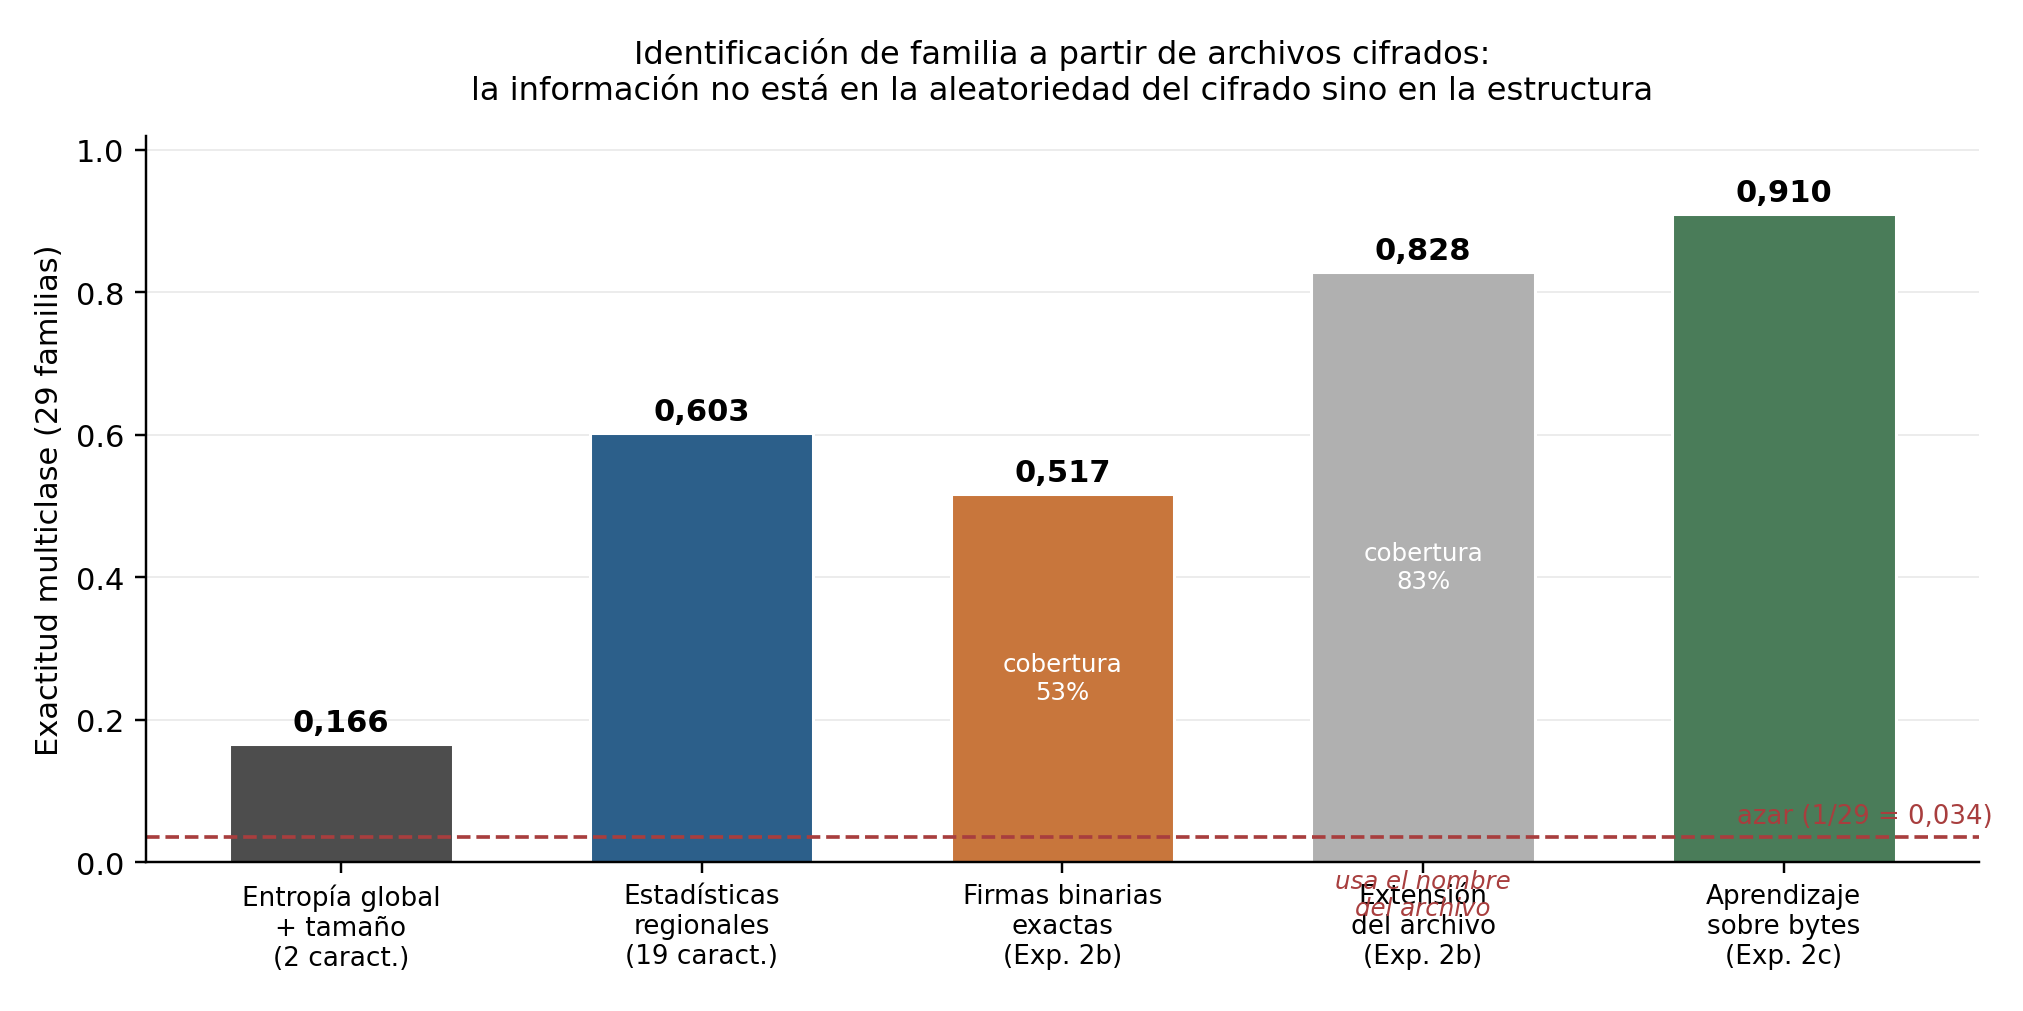
\includegraphics[width=0.95\textwidth]{images/fig_progresion_archivos.png}
\caption{Progresión de enfoques para la identificación de familia a partir de archivos cifrados. Cada enfoque responde a una limitación del anterior. El valor de la extensión se muestra en gris por tratarse de un identificador de campaña.}
\label{fig:progresion}
\end{figure}

Cada etapa responde a una objeción de la anterior: la ampliación del espacio de características descarta que el resultado negativo inicial se debiera a una representación pobre; la localización explícita de firmas identifica dónde reside la señal; y el aprendizaje sobre bytes extiende esa señal a la totalidad del conjunto sin recurrir a metadatos del nombre.

La conclusión del frente de archivos cifrados queda, por tanto, acotada con precisión: la indistinguibilidad estadística es real, pero se limita a \textbf{seis de las veintinueve familias evaluadas}, aquellas que cifran sin dejar estructura reconocible. Para las veintitrés restantes la información de familia está presente en el contenido del archivo y es extraíble automáticamente con una exactitud del 0,910.

\section{Experimento 3: Clasificación por Notas de Rescate (NLP)}
\label{sec:exp3}

\subsection{Variabilidad del Corpus: las Notas como Plantillas}
\label{subsec:res_variabilidad}

El análisis de casi-duplicados (Sección~\ref{subsec:neardups}) revela un fenómeno central para interpretar los resultados: \textbf{las 146 notas del corpus contienen solo 95 grupos de contenido distinto}. Las notas de rescate son plantillas que cada familia reutiliza modificando únicamente datos de contacto o identificadores de víctima. Los casos extremos son ilustrativos: las 19 notas de DHARMA corresponden a solo 6 plantillas (el mismo texto con distinta dirección de correo), las 18 de CERBER a 8, y las 4 de WASTEDLOCKER a una única plantilla.

Esta baja variabilidad intra-familia tiene dos consecuencias metodológicas: fundamenta el uso de los dos protocolos de evaluación (P1 y P2), y demuestra que la expansión del corpus debe medirse en \textit{plantillas} nuevas por familia, no solo en cantidad de archivos.

\subsection{Resultados bajo el Protocolo P1 (plantilla conocida)}

La Tabla~\ref{tab:exp3_p1} presenta los resultados del protocolo P1, que mide la capacidad de identificar la familia de una nueva instancia de una plantilla ya catalogada.

\begin{table}[ht]
\centering
\caption{Clasificación NLP bajo el protocolo P1 (146 notas, 30 familias, 2-fold CV $\times$ 10 semillas)}
\label{tab:exp3_p1}
\resizebox{\textwidth}{!}{
\begin{tabular}{|l|l|c|c|c|c|}
\hline
\textbf{TF-IDF} & \textbf{Modelo} & \textbf{Accuracy} & \textbf{Balanced acc.} & \textbf{Macro-F1} & \textbf{Weighted-F1} \\
\hline
\multirow{4}{*}{Palabras (1-2)} & LinearSVC & 0,821 & 0,770 & 0,748 $\pm$ 0,032 & 0,799 \\
 & Reg. Logística & 0,790 & 0,759 & 0,728 $\pm$ 0,029 & 0,770 \\
 & Random Forest & 0,749 & 0,664 & 0,660 $\pm$ 0,034 & 0,717 \\
 & KNN & 0,678 & 0,535 & 0,488 $\pm$ 0,032 & 0,632 \\
\hline
\multirow{4}{*}{Caracteres (3-5)} & LinearSVC & 0,818 & \textbf{0,777} & \textbf{0,760 $\pm$ 0,029} & 0,798 \\
 & Reg. Logística & 0,791 & 0,763 & 0,733 $\pm$ 0,035 & 0,769 \\
 & Random Forest & 0,745 & 0,645 & 0,626 $\pm$ 0,036 & 0,707 \\
 & KNN & 0,671 & 0,523 & 0,481 $\pm$ 0,025 & 0,626 \\
\hline
\multirow{4}{*}{Combinado} & LinearSVC & \textbf{0,825} & 0,769 & 0,754 $\pm$ 0,033 & \textbf{0,804} \\
 & Reg. Logística & 0,803 & 0,760 & 0,739 $\pm$ 0,031 & 0,782 \\
 & Random Forest & 0,753 & 0,660 & 0,647 $\pm$ 0,025 & 0,719 \\
 & KNN & 0,691 & 0,542 & 0,503 $\pm$ 0,026 & 0,647 \\
\hline
\end{tabular}
}
\end{table}

La mejor configuración por macro-F1 fue LinearSVC con n-gramas de caracteres (3-5): \textbf{macro-F1 de 0,760, balanced accuracy de 0,777 y accuracy de 0,818} sobre 30 clases, donde el azar equivale a 0,033. Los modelos lineales superan consistentemente a Random Forest y KNN, en línea con la efectividad conocida de los clasificadores lineales en espacios TF-IDF de alta dimensionalidad con pocas muestras~\cite{joachims1998}.

\subsection{Resultados bajo el Protocolo P2 (variante nunca vista)}

La Tabla~\ref{tab:exp3_p2} presenta los resultados del protocolo P2, en el que ninguna variante casi idéntica de una nota de prueba estuvo disponible durante el entrenamiento.

\begin{table}[ht]
\centering
\caption{Clasificación NLP bajo el protocolo P2 (grupos de casi-duplicados no repartidos, 2-fold CV $\times$ 10 semillas)}
\label{tab:exp3_p2}
\resizebox{\textwidth}{!}{
\begin{tabular}{|l|l|c|c|c|c|}
\hline
\textbf{TF-IDF} & \textbf{Modelo} & \textbf{Accuracy} & \textbf{Balanced acc.} & \textbf{Macro-F1} & \textbf{Weighted-F1} \\
\hline
\multirow{4}{*}{Palabras (1-2)} & LinearSVC & 0,535 & 0,481 & 0,422 $\pm$ 0,055 & 0,497 \\
 & Reg. Logística & 0,520 & 0,475 & 0,412 $\pm$ 0,050 & 0,479 \\
 & Random Forest & 0,486 & 0,393 & 0,363 $\pm$ 0,048 & 0,449 \\
 & KNN & 0,408 & 0,289 & 0,259 $\pm$ 0,026 & 0,374 \\
\hline
\multirow{4}{*}{Caracteres (3-5)} & LinearSVC & 0,529 & 0,470 & 0,412 $\pm$ 0,041 & 0,490 \\
 & Reg. Logística & 0,523 & 0,467 & 0,401 $\pm$ 0,048 & 0,483 \\
 & Random Forest & 0,484 & 0,383 & 0,348 $\pm$ 0,043 & 0,442 \\
 & KNN & 0,413 & 0,293 & 0,262 $\pm$ 0,036 & 0,384 \\
\hline
\multirow{4}{*}{Combinado} & LinearSVC & \textbf{0,551} & \textbf{0,492} & \textbf{0,435 $\pm$ 0,057} & \textbf{0,512} \\
 & Reg. Logística & 0,526 & 0,473 & 0,417 $\pm$ 0,051 & 0,488 \\
 & Random Forest & 0,497 & 0,397 & 0,364 $\pm$ 0,052 & 0,454 \\
 & KNN & 0,418 & 0,296 & 0,274 $\pm$ 0,045 & 0,392 \\
\hline
\end{tabular}
}
\end{table}

La mejor configuración fue la representación combinada con LinearSVC: \textbf{macro-F1 de 0,435 y accuracy de 0,551}. La caída respecto de P1 (de 0,760 a 0,435 en macro-F1) cuantifica exactamente cuánto del rendimiento aparente proviene de reconocer plantillas ya vistas: es una consecuencia directa de la baja variabilidad documentada en la Sección~\ref{subsec:res_variabilidad}, no un defecto del clasificador. Bajo P2 la representación combinada (palabras + caracteres) sí aporta una mejora sobre caracteres solos, lo que sugiere que ante variantes nuevas la información semántica y la morfológica se complementan.

\subsection{Análisis por Familia}

La Tabla~\ref{tab:exp3_familia} presenta el F1 por familia de la mejor configuración bajo P2, junto con el número de notas y de grupos de contenido distinto, y la Figura~\ref{fig:confusion_canonica} la matriz de confusión correspondiente.

\begin{table}[ht]
\centering
\caption{F1 por familia bajo P2 (combinado + LinearSVC, promedio de 10 semillas), ordenado descendentemente}
\label{tab:exp3_familia}
\resizebox{\textwidth}{!}{
\begin{tabular}{|l|c|c|c||l|c|c|c|}
\hline
\textbf{Familia} & \textbf{Notas} & \textbf{Grupos} & \textbf{F1} & \textbf{Familia} & \textbf{Notas} & \textbf{Grupos} & \textbf{F1} \\ \hline
AVOSLOCKER & 3 & 3 & 0,861 & SUNCRYPT & 2 & 2 & 0,500 \\ \hline
CERBER & 18 & 8 & 0,831 & DHARMA & 19 & 6 & 0,483 \\ \hline
GANDCRAB & 9 & 5 & 0,831 & LOCKBIT & 8 & 6 & 0,450 \\ \hline
CONTI & 4 & 3 & 0,786 & SODINOKIBI & 3 & 3 & 0,449 \\ \hline
BLACKCAT & 4 & 4 & 0,767 & CLOP & 4 & 4 & 0,378 \\ \hline
TESLACRYPT & 9 & 4 & 0,717 & BADRABBIT & 2 & 2 & 0,270 \\ \hline
LORENZ & 3 & 3 & 0,685 & HELLOKITTY & 5 & 5 & 0,248 \\ \hline
RANSOMEXX & 5 & 4 & 0,658 & CRYPTOLOCKER & 4 & 3 & 0,234 \\ \hline
BLACKMATTER & 2 & 2 & 0,650 & JIGSAW & 2 & 2 & 0,230 \\ \hline
PHOBOS & 4 & 4 & 0,637 & BLACKBASTA & 5 & 4 & 0,215 \\ \hline
DARKSIDE & 3 & 2 & 0,603 & NOTPETYA & 2 & 2 & 0,197 \\ \hline
CUBA & 4 & 2 & 0,589 & RYUK & 4 & 2 & 0,075 \\ \hline
NETWALKER & 3 & 2 & 0,586 & CHIMERA & 2 & 2 & 0,067 \\ \hline
 & & & & MEDUZALOCKER & 4 & 3 & 0,065 \\ \hline
 & & & & WANNACRY & 2 & 2 & 0,000 \\ \hline
 & & & & MAZE & 3 & 2 & 0,000 \\ \hline
 & & & & WASTEDLOCKER & 4 & 1 & 0,000 \\ \hline
\end{tabular}
}
\end{table}

\begin{figure}[ht]
\centering
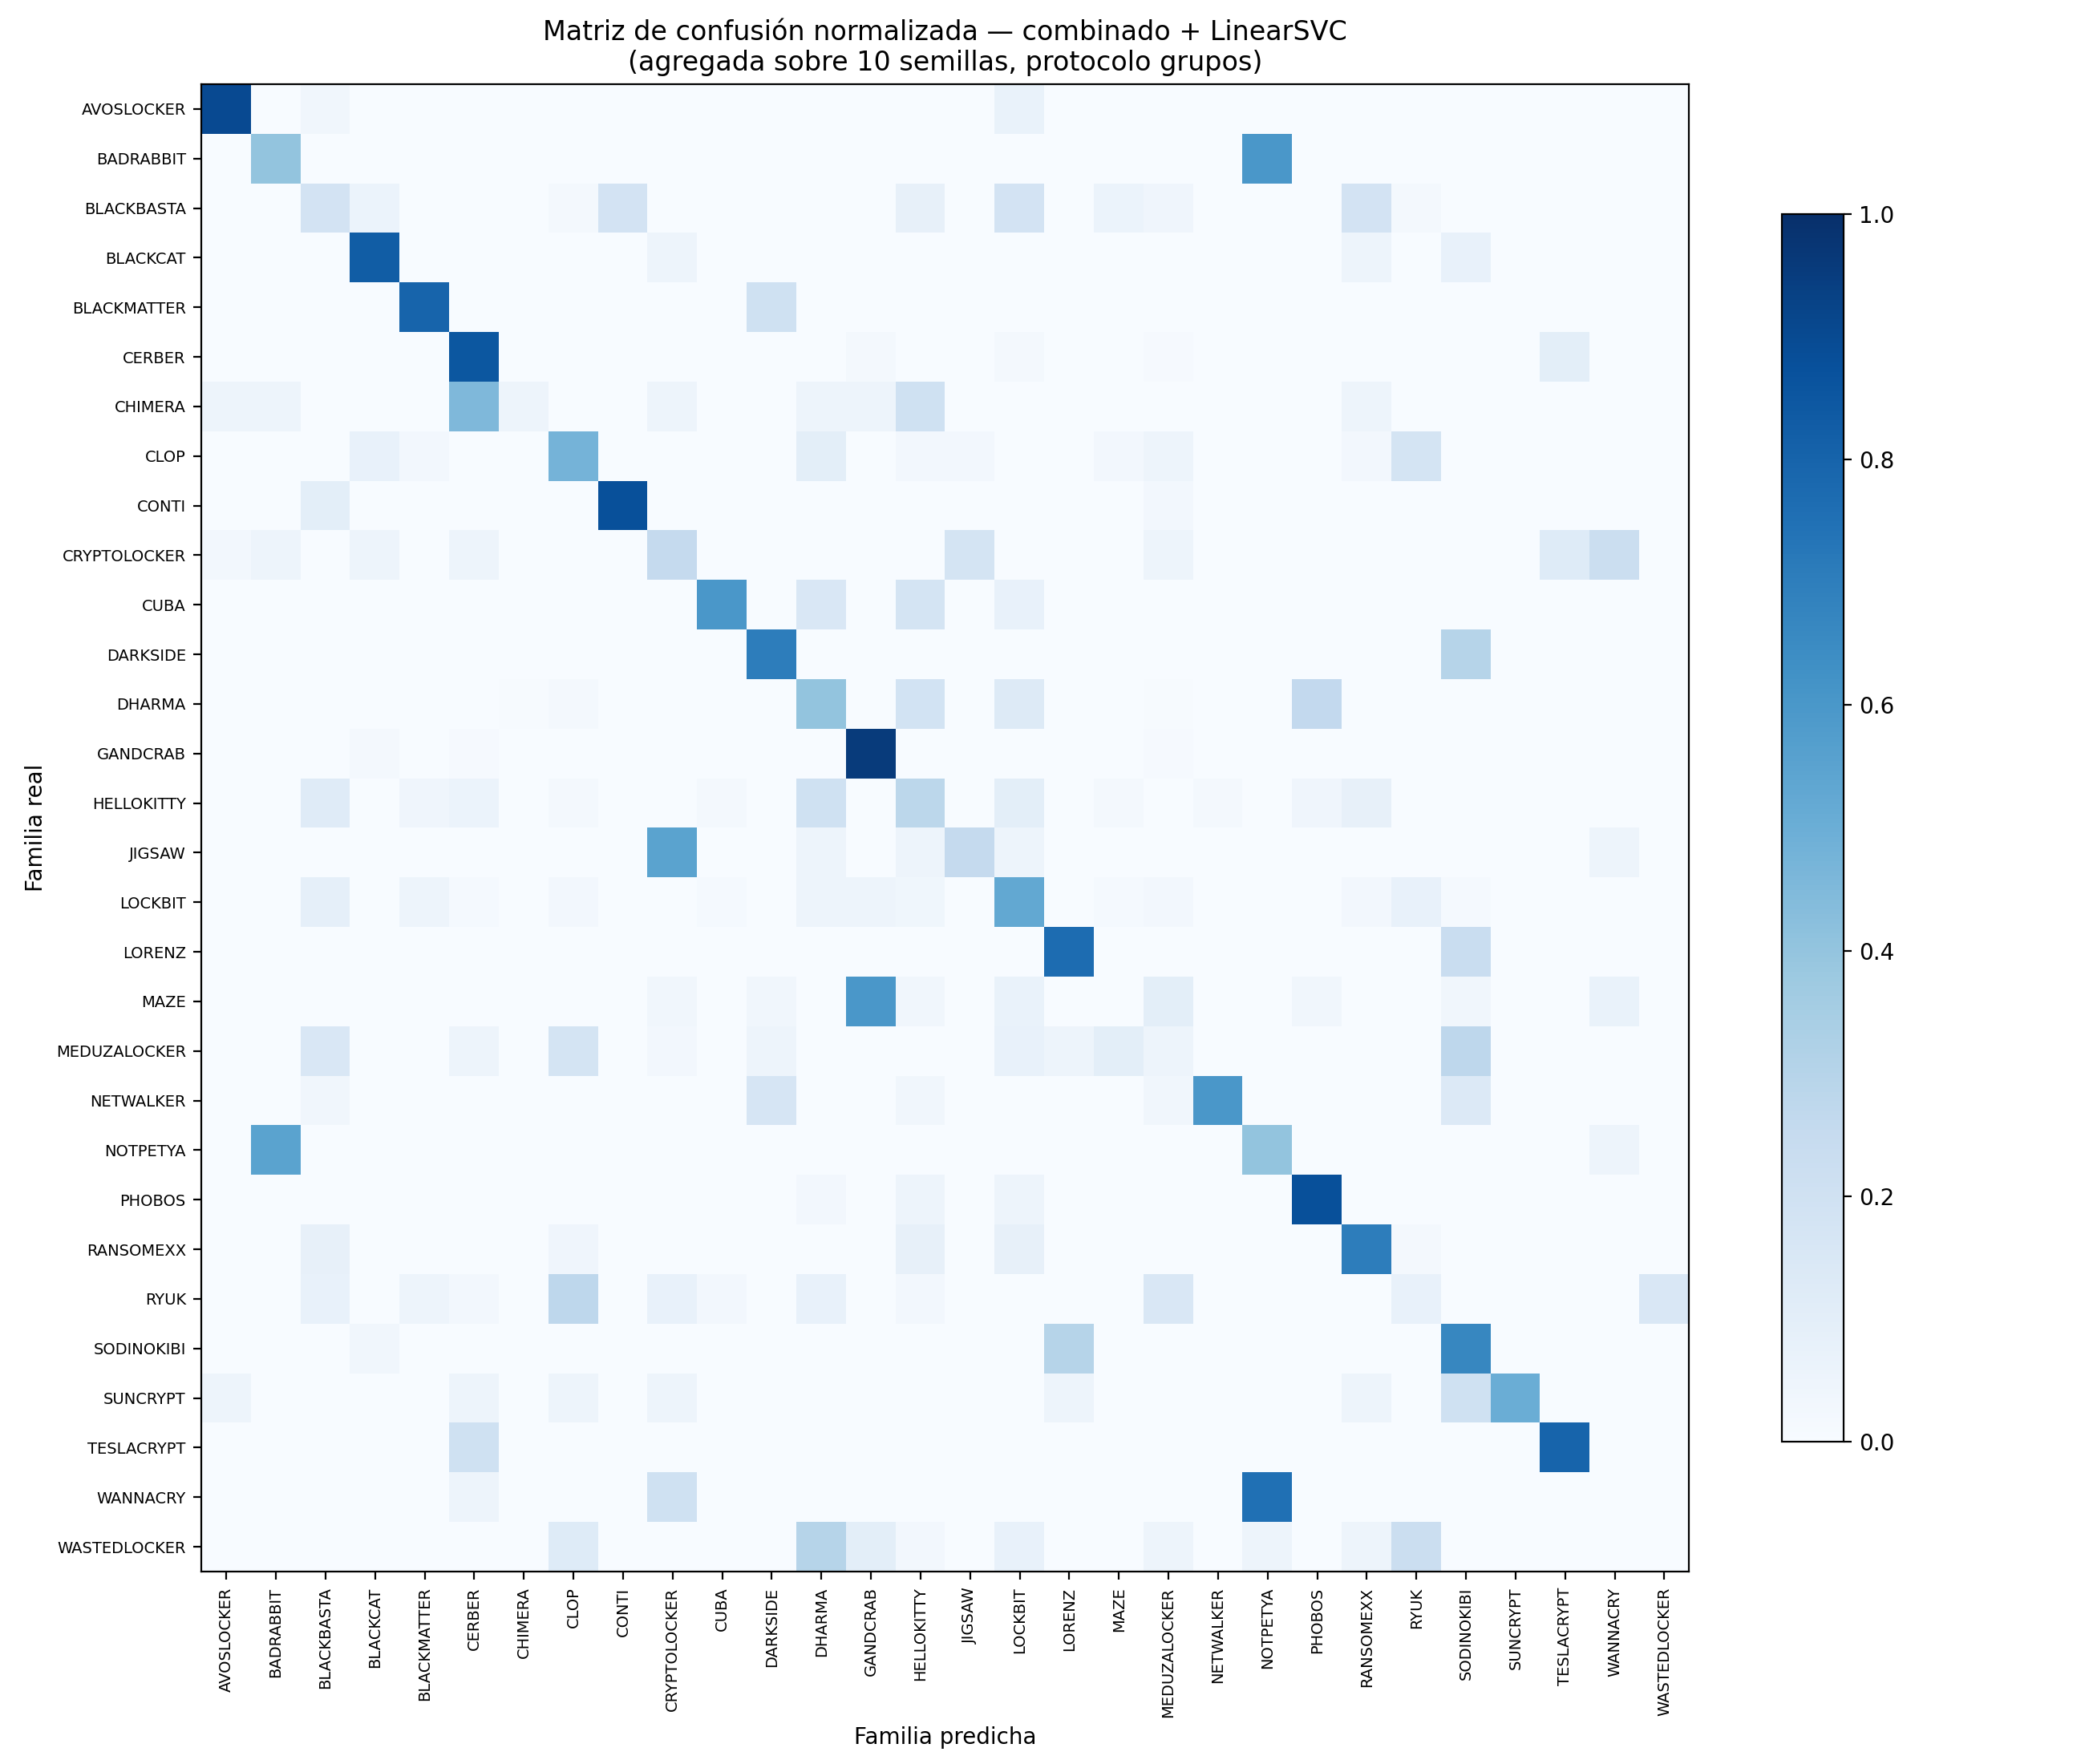
\includegraphics[width=0.95\textwidth]{images/fig_confusion_canonica.png}
\caption{Matriz de confusión normalizada de la mejor configuración bajo P2 (combinado + LinearSVC), agregada sobre las 10 repeticiones.}
\label{fig:confusion_canonica}
\end{figure}

Se observa un patrón claro: las familias con mayor diversidad de plantillas y notas extensas y distintivas (AVOSLOCKER, CERBER, GANDCRAB, CONTI, BLACKCAT) se clasifican bien incluso ante variantes nuevas, mientras que las familias con pocas plantillas o notas muy breves y genéricas (WANNACRY, MAZE, CHIMERA, RYUK) no logran generalizarse. WASTEDLOCKER constituye el caso límite: sus 4 notas forman un único grupo de contenido, por lo que bajo P2 es estructuralmente inevaluable (F1 = 0 por construcción, declarado en la Sección~\ref{subsec:protocolos_nlp}).

Este patrón converge con las observaciones de Lemmou et al.~\cite{paper_5_note_files}, cuyos falsos positivos de similitud de contenido corresponden precisamente a confusiones entre familias emparentadas (CryptoLocker con TeslaCrypt, entre otras): la dificultad de atribuir familia ante contenido nuevo o compartido es una propiedad del dominio, no un defecto del método.

\subsection{Optimización de hiperparámetros}
\label{subsec:exp3_hiperparametros}

Los resultados anteriores se obtuvieron con la configuración por defecto de cada modelo. Para descartar que el rendimiento estuviera limitado por una elección subóptima de parámetros ---objeción habitual ante un resultado que no alcanza los valores deseados--- se realizó una búsqueda sistemática sobre 360 configuraciones para la representación de palabras y 480 para la de caracteres, variando el rango de n-gramas, el tamaño máximo del vocabulario, los umbrales de frecuencia documental y el parámetro de regularización $C$.

La búsqueda se implementó de forma \textbf{anidada}: para cada partición externa, la selección de hiperparámetros se realiza mediante validación cruzada interna sobre el subconjunto de entrenamiento, y la evaluación se efectúa sobre la partición externa, que no participó de la selección. Este diseño evita el sesgo optimista que introduce elegir la configuración observando el mismo conjunto sobre el que después se reporta el resultado. El procedimiento se repitió con las diez semillas y bajo ambos protocolos.

\begin{table}[ht]
\centering
\caption{Clasificación de notas con hiperparámetros optimizados (búsqueda anidada, 144 notas, 10 semillas)}
\label{tab:exp3_hiperparametros}
\begin{tabular}{|l|c|c|}
\hline
\textbf{Configuración} & \textbf{P1 (plantilla conocida)} & \textbf{P2 (variante nueva)} \\
\hline
Palabras + LinearSVC & 0,754 $\pm$ 0,029 & 0,408 $\pm$ 0,052 \\
Palabras + Reg. Logística & 0,734 $\pm$ 0,030 & 0,400 $\pm$ 0,054 \\
Caracteres + LinearSVC & 0,742 $\pm$ 0,050 & 0,416 $\pm$ 0,060 \\
Caracteres + Reg. Logística & 0,737 $\pm$ 0,039 & 0,407 $\pm$ 0,065 \\
\textbf{Combinado, mejores hiperparámetros} & \textbf{0,775 $\pm$ 0,032} & \textbf{0,424 $\pm$ 0,064} \\
\hline
\end{tabular}
\end{table}

\textbf{La optimización no produce una mejora significativa.} Los valores obtenidos (macro-F1 de 0,775 bajo P1 y 0,424 bajo P2) son estadísticamente indistinguibles de los alcanzados con la configuración por defecto, dado que las diferencias caen dentro del desvío estándar entre semillas.

Este resultado negativo es informativo. Indica, en primer lugar, que la configuración adoptada inicialmente ---n-gramas de caracteres de 3 a 5 con LinearSVC, siguiendo la práctica establecida para clasificación de texto en espacios de alta dimensionalidad y datos dispersos~\cite{joachims1998}--- era ya adecuada para el problema. Y señala, en segundo lugar, que \textbf{el factor limitante no es la parametrización del modelo sino la composición del corpus}: con 95 plantillas distintas repartidas entre 30 familias, y siete de ellas representadas por una sola plantilla, ningún ajuste de hiperparámetros puede suplir la ausencia de ejemplos. La ampliación del corpus en profundidad queda así respaldada cuantitativamente, y no como mera recomendación.

\subsection{Comparación con los Resultados Previos del Proyecto}
\label{subsec:res_escalera}

En etapas anteriores del trabajo se reportó una accuracy del 89,7\% (macro-F1 0,840) sobre el corpus original de 156 notas. La Tabla~\ref{tab:escalera} desglosa la transición hacia los valores canónicos, en aras de la transparencia metodológica.

\begin{table}[ht]
\centering
\caption{Evolución de los resultados del Experimento 3 al corregir el protocolo de evaluación}
\label{tab:escalera}
\resizebox{\textwidth}{!}{
\begin{tabular}{|l|c|c|l|}
\hline
\textbf{Corrida} & \textbf{Accuracy} & \textbf{Macro-F1} & \textbf{Factores corregidos} \\
\hline
Corpus original (156 notas) & 0,897 & 0,840 & --- (24\% de notas duplicadas; fuga de vocabulario; \\
 & & & codificación UTF-16 mal leída; 1 semilla) \\
\hline
Canónica, protocolo P1 & 0,818 & 0,760 & deduplicación, codificación, \textit{pipeline} sin fuga, \\
 & & & 10 semillas \\
\hline
Canónica, protocolo P2 & 0,551 & 0,435 & + plantillas casi idénticas nunca repartidas \\
 & & & entre entrenamiento y prueba \\
\hline
\end{tabular}
}
\end{table}

Cada corrección reduce el valor nominal pero aumenta la validez: el 0,897 original medía en parte la capacidad del modelo de reconocer notas duplicadas; el protocolo P1 mide el reconocimiento de nuevas instancias de plantillas conocidas; y el protocolo P2, la generalización a contenido nunca visto.

\section{Ajustes al Protocolo Experimental}
\label{sec:ajustes_protocolo}

El diseño experimental presentado no se alcanzó de una sola vez. Durante la ejecución del trabajo se detectaron y corrigieron varios problemas que alteraban los resultados, y se documentan aquí por dos razones: porque las cifras previas a cada corrección circularon en informes de avance del proyecto, y porque varios de estos problemas son errores frecuentes cuya descripción puede resultar útil a trabajos similares.

\subsection{Detección de la codificación de las notas}

Catorce de las notas del corpus, pertenecientes a las familias DHARMA, GANDCRAB y SUNCRYPT, no están codificadas en UTF-8 sino en UTF-16 o cp1252. Las notas de rescate se generan en los equipos comprometidos, donde el editor predeterminado del sistema puede emplear codificaciones distintas, de modo que esta heterogeneidad es un rasgo del artefacto y no un defecto de la recolección.

La lectura de un archivo UTF-16 asumiendo UTF-8 no produce error: genera texto con bytes nulos intercalados entre los caracteres. El efecto fue doble y de signo contrario. Por un lado, trece notas ---el 8,9\% del corpus--- ingresaban al vectorizador de palabras como documentos vacíos. Por otro, en la representación de caracteres esos bytes nulos constituían una secuencia exclusiva de DHARMA y GANDCRAB, es decir, una firma sintética que el clasificador aprendía como si fuera un rasgo de esas familias. El procedimiento de lectura se modificó para detectar la codificación real de cada archivo (marca de orden de bytes, heurística de proporción de bytes nulos y retroceso a cp1252), tras lo cual ninguna nota ingresa vacía.

\subsection{Control de duplicados y casi-duplicados}

El corpus original contenía 156 notas correspondientes a 118 textos únicos: un 24\% de redundancia originada en que varias fuentes publican las mismas notas. Con una partición aleatoria, copias idénticas quedaban simultáneamente en entrenamiento y prueba, de modo que el clasificador era evaluado sobre documentos que ya había visto. La reconstrucción del corpus (\texttt{corpus\_v2}) eliminó los duplicados exactos, pero el análisis de similitud reveló que persistían pares casi idénticos ---variantes de una misma nota con distinta dirección de contacto---, lo que motivó el agrupamiento descrito en la Sección~\ref{subsec:neardups} y la adopción del protocolo P2.

\subsection{Fuga de información en la vectorización}

En la implementación inicial, el vectorizador TF-IDF se ajustaba sobre la totalidad del corpus antes de iniciar la validación cruzada. En consecuencia, el vocabulario y las frecuencias documentales inversas incorporaban información de los documentos de prueba. La corrección consistió en encapsular vectorizador y clasificador en un \texttt{Pipeline}~\cite{sklearn}, de modo que ambos se ajusten exclusivamente con el subconjunto de entrenamiento de cada partición, replicando la situación real de aplicación sobre una nota no vista previamente.

\subsection{Estabilidad de la estimación}

Con 144 documentos repartidos en 30 clases, una única partición aleatoria puede producir estimaciones no representativas. La validación se repite con diez semillas distintas y se reporta la media junto con el desvío estándar entre repeticiones, lo que permite además distinguir diferencias reales entre configuraciones de la variabilidad propia del muestreo, como fue el caso en el análisis de hiperparámetros (Sección~\ref{subsec:exp3_hiperparametros}).

\subsection{Selección de métricas}

Los informes iniciales del proyecto reportaban un 87,58\% que correspondía a la exactitud global, acompañada de métricas promediadas de forma ponderada por el tamaño de cada clase. Dado que las dos familias más numerosas concentran el 25\% del corpus, ese promedio queda dominado por ellas y sobreestima el rendimiento sobre las familias pequeñas, que son precisamente las de mayor interés operativo. Se adoptó en consecuencia el macro-F1 como métrica principal, acompañado de la exactitud balanceada, el informe por familia y la matriz de confusión. La diferencia entre ambos promedios ---0,798 ponderado frente a 0,760 macro bajo el protocolo P1--- cuantifica el sesgo.

\subsection{Ejecución en infraestructura compartida}

Los experimentos sobre el conjunto completo de NapierOne se ejecutaron en el clúster computacional del NIDTEC, gestionado mediante SLURM. Tres trabajos fueron cancelados por el sistema antes de completarse, por causas relacionadas entre sí que se documentan por su valor práctico: la asignación de memoria por defecto (2 GB) resulta insuficiente y debe solicitarse de forma explícita; la configuración \texttt{n\_jobs=-1}, habitual en un equipo personal, reserva la totalidad de los núcleos del nodo en lugar de los asignados al trabajo, por lo que se sustituyó por la lectura de la variable de entorno correspondiente; y la combinación de paralelismo en la validación cruzada con paralelismo interno del modelo generaba una multiplicación de procesos, cada uno con su propia copia de la matriz de características. Corregidos estos aspectos, la extracción de características sobre 29.029 archivos requirió 5,5 horas y el entrenamiento posterior 20 minutos.

\section{Evaluación de Herramientas Existentes}
\label{sec:res_herramientas}

La Tabla~\ref{tab:herramientas} resume la evaluación experimental de CryptoSheriff~\cite{cryptosheriff} e ID Ransomware~\cite{idransomware} descrita en la Sección~\ref{sec:met_herramientas}.

\begin{table}[ht]
\centering
\caption{Evaluación experimental de herramientas públicas de identificación de ransomware}
\label{tab:herramientas}
\begin{tabular}{|l|l|c|}
\hline
\textbf{Herramienta} & \textbf{Entrada} & \textbf{Identificación correcta} \\
\hline
CryptoSheriff & Archivos cifrados (30 familias) & 5/30 (16,67\%) \\
ID Ransomware & Archivos cifrados (30 familias) & 20/30 (66,67\%) \\
ID Ransomware & Notas de rescate (57 notas, 22 familias) & 41/57 (71,93\%) \\
\hline
\end{tabular}
\end{table}

De las 20 familias que ID Ransomware identifica por archivo cifrado, 9 mantienen la identificación al renombrar el archivo (GANDCRAB, LORENZ, MAZE, MEDUSALOCKER, PHOBOS, RYUK, SODINOKIBI, TESLACRYPT y WANNACRY): en esos casos la herramienta reconoce firmas de bytes o metadatos que la familia inserta en el archivo cifrado. En las 11 restantes, la identificación depende del patrón del nombre o la extensión. Este resultado es consistente con el hallazgo del Experimento~2: la identificación de familia a partir del archivo cifrado solo es posible cuando la familia deja marcas deliberadas, no por propiedades estadísticas del cifrado.

\section{Comparación entre Enfoques}

La Tabla~\ref{tab:comparacion_final} integra los resultados de los tres experimentos y de la evaluación de herramientas.

\begin{table}[ht]
\centering
\caption{Comparación de los enfoques evaluados}
\label{tab:comparacion_final}
\resizebox{\textwidth}{!}{
\begin{tabular}{|l|c|c|l|}
\hline
\textbf{Enfoque} & \textbf{Clases} & \textbf{Resultado} & \textbf{Mejor método} \\
\hline
Exp. 1: Binaria (archivos) & 2 & 88,6\% acc. & Random Forest \\
Exp. 2: Multiclase, 2 características & 31 & 9,9\% acc. & Gradient Boosting \\
Exp. 2: Multiclase, 19 características & 29 & 60,3\% acc. & Random Forest \\
Exp. 2b: Firmas binarias (donde aplican) & 29 & 97,0\% acc. (53\% cobert.) & Coincidencia exacta \\
Exp. 2c: Aprendizaje sobre bytes & 29 & \textbf{91,0\% acc. / 0,908 macro-F1} & Random Forest (posicional) \\
Exp. 3: NLP notas, P1 (plantilla conocida) & 30 & 81,8\% acc. / 0,760 macro-F1 & LinearSVC (caracteres) \\
Exp. 3: NLP notas, P2 (variante nueva) & 30 & 55,1\% acc. / 0,435 macro-F1 & LinearSVC (combinado) \\
\hline
ID Ransomware (notas) & --- & 71,93\% & Reglas manuales \\
ID Ransomware (archivos) & --- & 66,67\% & Reglas y \textit{magic bytes} \\
CryptoSheriff (archivos) & --- & 16,67\% & Reglas manuales \\
\hline
\end{tabular}
}
\end{table}

Los resultados demuestran que:

\begin{enumerate}
    \item Las métricas estadísticas de archivos cifrados son efectivas para la \textbf{detección binaria} de cifrado ($\sim$89\% de exactitud).
    \item La \textbf{identificación de familia a partir de archivos cifrados es posible} (91,0\% de exactitud sobre 29 familias, sin emplear metadatos del nombre), pero no mediante las propiedades criptográficas del contenido, sino a través de los artefactos estructurales que cada familia añade. La indistinguibilidad se limita a seis familias que cifran sin dejar estructura reconocible.
    \item Las notas de rescate permiten la identificación de familia con 81,8\% de exactitud en el escenario operativo comparable al de las herramientas existentes (P1), superando el 71,93\% de ID Ransomware, con la ventaja adicional de constituir un método automático y reproducible frente a reglas mantenidas manualmente.
    \item La generalización a variantes nunca vistas (P2, macro-F1 0,435) es sustancialmente más difícil y depende de la diversidad de plantillas disponible por familia, lo que fundamenta la expansión del corpus como línea de trabajo prioritaria.
\end{enumerate}

\section{Discusión}

\subsection{Una misma lección desde dos artefactos distintos}

Los dos frentes del trabajo, desarrollados de forma independiente y sobre datos de naturaleza muy distinta, convergen en una observación común que constituye el aporte conceptual de esta tesis: en ambos casos existe una señal fácil de explotar pero ligada a la campaña concreta, y una señal más difícil pero propia del contenido, y ambas no deben confundirse.

\begin{figure}[ht]
\centering
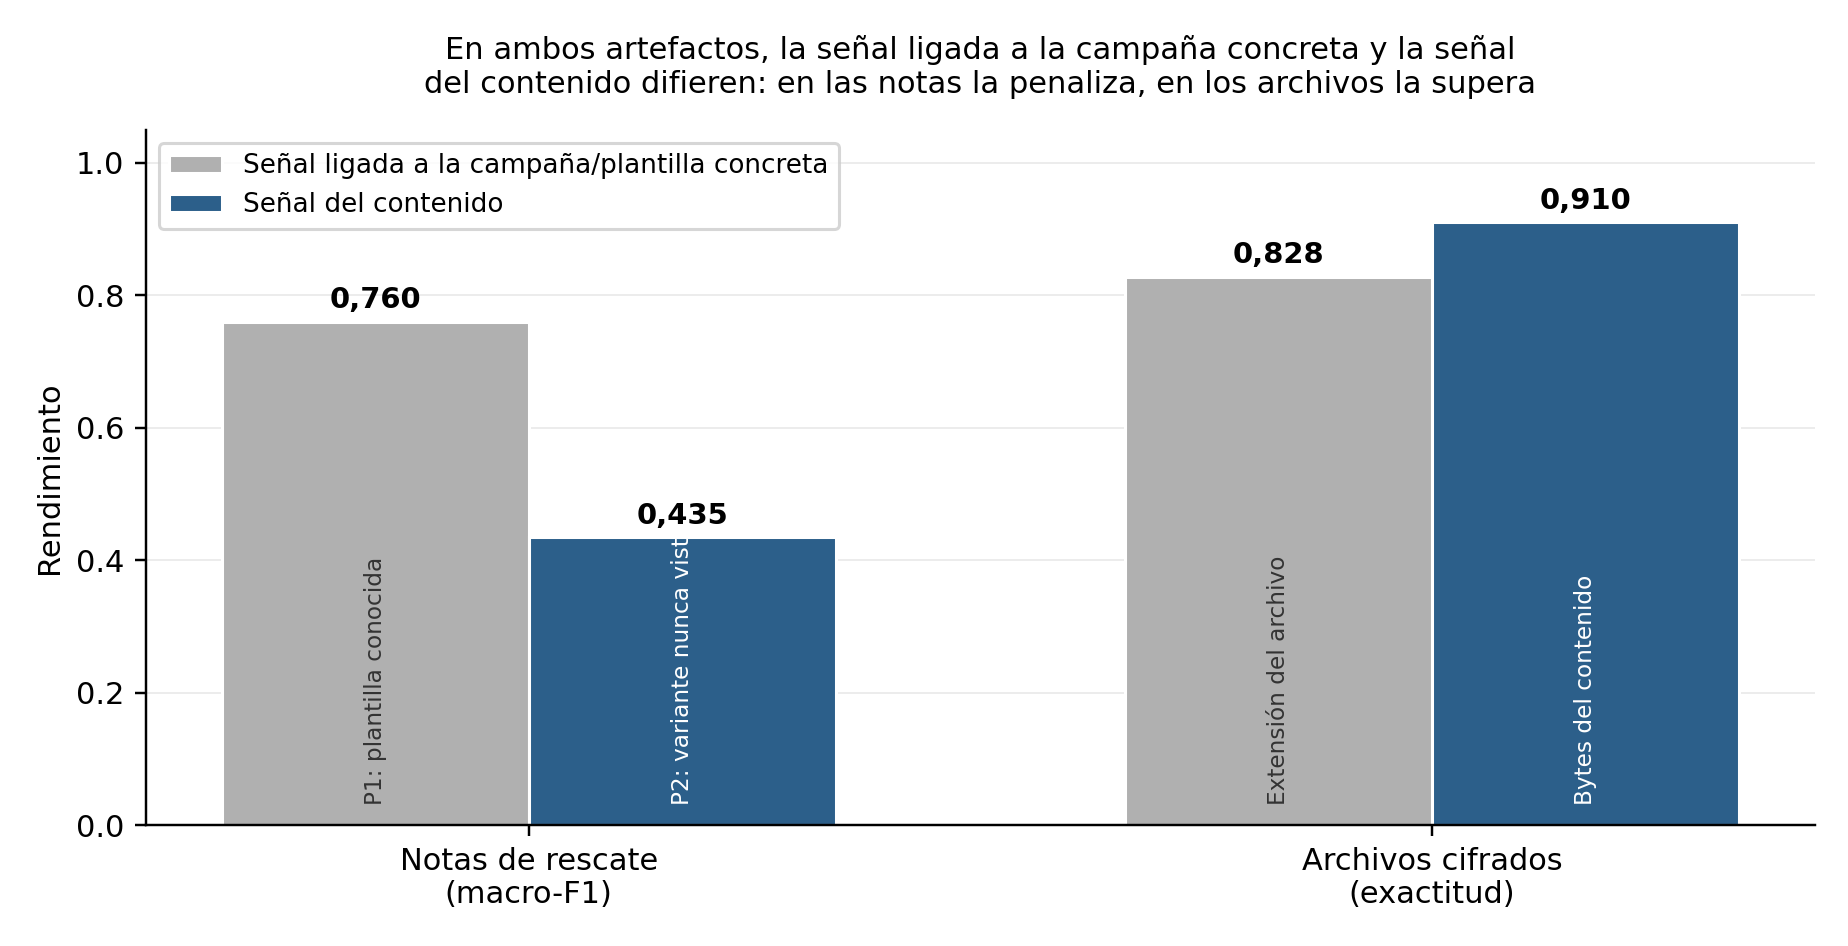
\includegraphics[width=0.92\textwidth]{images/fig_simetria_frentes.png}
\caption{Comparación entre la señal ligada a la campaña o plantilla concreta y la señal del contenido, en los dos artefactos analizados.}
\label{fig:simetria}
\end{figure}

En las \textbf{notas de rescate}, la señal fácil es la plantilla: reconocer una nueva instancia de un texto ya catalogado alcanza un macro-F1 de 0,760, mientras que atribuir una variante nunca vista desciende a 0,435. En los \textbf{archivos cifrados}, la señal fácil es la extensión añadida, que acierta el 100\% de los casos en que está presente pero identifica la campaña y no la familia; la señal de contenido, en cambio, alcanza 0,910 y resulta más estable porque proviene de marcadores que el propio programa escribe en el archivo.

Esta distinción explica por qué las herramientas basadas en catálogos de reglas, como ID Ransomware~\cite{idransomware} o el identificador propuesto por Lemmou et al.~\cite{paper_5_note_files}, funcionan satisfactoriamente sobre campañas conocidas y requieren actualización permanente: operan sobre la señal fácil. Un clasificador entrenado sobre el contenido no las reemplaza, pero cubre el caso que ellas no resuelven, que es precisamente el de las variantes no catalogadas.

\subsection{Implicaciones para el análisis post-ataque}

Los resultados permiten proponer un procedimiento por etapas en el que cada artefacto cumple la función para la que resulta adecuado:

\begin{enumerate}
\item \textbf{Confirmación del incidente} mediante métricas estadísticas sobre los archivos afectados (detección binaria, $\sim$89\% de exactitud). Los archivos cifrados son el único artefacto cuya presencia está garantizada: la nota puede haber sido eliminada, no encontrada, o directamente no existir.
\item \textbf{Identificación de familia por el contenido del archivo cifrado} (91,0\%), aplicable a las 23 familias que añaden estructura reconocible.
\item \textbf{Identificación de familia por la nota de rescate} cuando esté disponible (81,8\% en el escenario comparable con las herramientas existentes), especialmente valiosa para las seis familias que no dejan estructura en los archivos.
\end{enumerate}

\subsection{Sobre la naturaleza de los resultados negativos}

El planteamiento inicial de este trabajo sostenía que las propiedades estadísticas de los archivos cifrados no permiten distinguir familias. La ampliación del espacio de características mostró que esa formulación era demasiado amplia: lo indistinguible es la aleatoriedad del contenido cifrado, no el archivo en su conjunto. Conviene señalar que el resultado negativo original no era erróneo sino insuficientemente delimitado, y que su delimitación precisa ---seis familias de veintinueve--- resulta más informativa que la afirmación general de la que se partió.

Un caso análogo se presenta en el análisis de hiperparámetros de la Sección~\ref{subsec:exp3_hiperparametros}: la ausencia de mejora tras una búsqueda sistemática es en sí misma un resultado, porque desplaza la explicación del rendimiento desde la parametrización del modelo hacia la composición del corpus, que es donde efectivamente se encuentra el factor limitante.

El hallazgo de que las notas de rescate son plantillas de baja variabilidad intra-familia (146 notas, 95 contenidos distintos) reformula el problema de clasificación: el desafío no es distinguir estilos de redacción, sino cubrir el repertorio de plantillas de cada familia. De ahí que el rendimiento bajo P2 esté fuertemente correlacionado con la diversidad de plantillas disponible, y que la expansión del corpus deba priorizarse en \textit{profundidad} (más plantillas por familia) antes que en cantidad de familias.

Finalmente, cabe señalar la importancia metodológica de las métricas elegidas: en un corpus donde dos familias concentran el 25\% de las notas, reportar únicamente accuracy o F1 ponderado sobrestimaría el rendimiento real. La diferencia entre el weighted-F1 (0,798) y el macro-F1 (0,760) bajo P1 ---y la brecha mayor bajo P2 (0,512 vs.\ 0,435)--- ilustra el sesgo que introducen las familias grandes, y justifica la adopción del macro-F1 como métrica principal.

Las limitaciones del estudio son el tamaño del corpus (146 notas, con 7 familias de solo 2 notas), la validación restringida a 2 folds por ese motivo, y la procedencia mixta de las notas (96 archivos brutos, 37 del corpus previo y 13 transcripciones), declarada nota por nota en el manifiesto del corpus.
